% =====================================================================
% Rolling-Governed Pinch Stability — RA-L submission, 6-page version
% Trimmed from main.tex (7 pages). All claims and numbers preserved;
% cuts are redundancy across sections + figure down-scaling.
% Compile: latexmk -pdf main_6p.tex   (or Overleaf)
% =====================================================================
\documentclass[journal]{IEEEtran}

\usepackage{graphicx}
\usepackage{amsmath,amssymb}
\usepackage{booktabs}
\usepackage[hidelinks]{hyperref}
\usepackage{balance}

\newcommand{\mueff}{\mu_{\mathrm{eff}}}
\newcommand{\mupair}{\mu_{\mathrm{pair}}}
\newcommand{\fstar}{f^{*}}
\newcommand{\repourl}{\url{https://github.com/NutcrackerWOW/Simplified-3D-Object-Manipulation-using-TacTip}}

\begin{document}

\title{Rolling-Governed Pinch Stability: A Validated Minimal Grip-Force
  Rule for Soft Tactile Fingertips}

\author{Jinxi Chen%
  \thanks{Manuscript received 06/07/2026; revised XXX. (Corresponding author:
    Author Name.)}%
  \thanks{The author is with Bristol Robotics Laboratory (e-mail: jinxichenhhh@gmail.com).}%
  \thanks{Code, models, and data are released at
    \protect\repourl.}%
}

\markboth{IEEE Robotics and Automation Letters. Preprint version.}%
{Jinxi Chen: Rolling-Governed Pinch Stability}

\maketitle

\begin{abstract}
Soft optical tactile fingertips such as the TacTip gain their sensitivity
from compliance, but the same compliance lets a pinched object \emph{roll}
off the fingertip domes below the Coulomb sliding limit. In a
compliant-hydroelastic simulation (Drake) of a two-finger pinch with
TacTip-style domes, we measure the minimal stable squeeze force $\fstar$
across grasp posture, object mass, shape, friction, and fingertip
stiffness. The stability boundary is rolling-governed: the effective
stability ratio $\mueff = (mg/2)/\fstar$ sits 25--35\,\% below the pair
Coulomb coefficient at every friction tested, so a friction-cone analysis
systematically underestimates the required force. Shape alone spans a
$2\times$ range of $\fstar$ at fixed friction, and softer fingertips reduce
$\mueff$ ($0.68 \to 0.49$, $100 \to 25$~kPa). Bootstrap analysis shows
$\mueff$ is statistically flat in posture inside the validity envelope; the
deployable rule is $\mueff \approx 0.71 - 4.2\,(m - 0.045)$ [$m$ in kg],
validated 16/16 on held-out posture--mass probes. Near the boundary, grasps
fail by slow rolling creep (5--11~s) with no vibration warning, motivating
a $\times 2.0$ force margin under which 30/30 seeded carry runs succeed; a
posture-scheduled threshold also makes a vibration slip detector deployable
at the sensor's 100~Hz camera rate. Code and data are publicly released.
\end{abstract}

\begin{IEEEkeywords}
Grasping, force and tactile sensing, contact modeling, simulation and
animation, grippers and other end-effectors.
\end{IEEEkeywords}

\IEEEpeerreviewmaketitle

\section{Introduction}

\IEEEPARstart{G}{rip} force selection is the most basic decision a
manipulating hand makes: squeeze too little and the object falls, squeeze
too much and the object is deformed, ejected, or energy is wasted. Sixty
years of grasp analysis provide the standard answer --- treat each contact
as a friction cone, require the load wrench to be resisted inside the
cones, and add an empirical safety margin. For rigid point contacts this is
essentially correct. But modern tactile fingertips are not rigid points:
sensors such as the TacTip family
\cite{chorley2009development,wardcherrier2018tactip} wrap a soft
hemispherical membrane around a camera, and the same compliance that gives
them their sensitivity gives the grasped object a new way to fail --- it
can \emph{roll} off the dome.

This paper quantifies that failure mode and turns the result into an
engineering rule. We build a simulation testbed around a two-finger hand
with compliant hydroelastic fingertip domes, pinching gravity-loaded
objects with the pinch axis horizontal so that weight loads the contacts in
shear (Fig.~\ref{fig:setup}). The testbed runs the
\emph{acquisition-to-hold} pipeline end to end, so we can locate the
minimal stable squeeze force $\fstar$ by bisection for any posture, object,
and material, and ask what actually sets it.

The answer is consistent across every sweep we ran: the boundary is
\textbf{rolling-governed}. At forces just below $\fstar$ the object does
not slide down the pads; it rotates about the grasp axis and escapes
(Fig.~\ref{fig:rolling}), and the effective stability ratio
$\mueff = (mg/2)/\fstar$ --- higher means a cheaper-to-hold grasp ---
saturates 25--35\,\% below the material pair's Coulomb coefficient at every
tested friction level. None of this is visible to a friction-cone
analysis, which predicts the same force for a sphere and a disc.

Rolling failure of soft contacts is qualitatively anticipated: the
soft-finger limit surface
\cite{goyal1991planar,kao1992quasistatic,xydas1999modeling} bounds the
coupled force--torque capacity of a compliant patch, and rotational
stability conditions have recently been derived for soft pneumatic fingers
\cite{jang2024rotational}. Our contribution is \emph{quantitative and
operational}:
\begin{enumerate}
  \item \textbf{Mechanism, quantified.} The pinch stability boundary for
    soft hemispherical fingertips is set by rolling, not Coulomb sliding:
    $\mueff$ sits 25--35\,\% below the pair friction at all tested
    frictions, geometry alone moves $\fstar$ by $2\times$ at fixed
    friction, and softer fingertips lower $\mueff$ from 0.68 (100~kPa) to
    0.49 (25~kPa) --- a direct sensitivity-versus-stability trade-off for
    soft tactile sensors.
  \item \textbf{A validated minimal grip-force rule.}
    $f_1^{*} = (mg/2)/\mueff$ with the one-line
    $\mueff \approx 0.71 - 4.2\,(m-0.045)$: bootstrap confidence intervals
    show the boundary is statistically flat in posture inside the validity
    envelope, so mass --- not posture --- carries the rule; it scores
    16/16 on held-out posture--mass probes (hold at $1.25\times$, drop at
    $0.6\times$).
  \item \textbf{Deployable slip-threshold calibration.} Over 90 episodes
    spanning the envelope, the pre-slip vibration floor varies up to
    $72\times$, so any single global threshold fails (0/30 detections at
    the only safe setting) although every slip burst clears its own
    condition's floor by ${\ge}3.6\times$; scheduling the threshold over
    $(\phi,\theta,m)$ recovers 30~TP\,/\,1~FP\,/\,0~FN\,/\,29~TN at both
    the ideal rate and the sensor's 100~Hz camera rate.
\end{enumerate}

We also show the measured boundary is \textbf{hold-duration-dependent}: at
$1.3\times\fstar$ the grasp survives the classic 3~s test window but fails
at 5.3--11.1~s by slow rolling creep --- motionless or carried alike
(\S\ref{sec:carried}), converged in the solver time step --- with no
vibration warning: the $\times 2.0$ margin in our rule is a measured
requirement, not conservatism. The study is simulation-only by design:
hydroelastic contact gives a controlled, converged testbed in which
$\fstar$ is measurable to a few percent and 2{,}100-trial sweeps are
tractable; \S\ref{sec:limitations} details what the idealization does and
does not cover.

\section{Related Work}

\textbf{Soft-finger contact and limit surfaces.} The limit-surface
formalism \cite{goyal1991planar,kao1992quasistatic,xydas1999modeling}
bounds a compliant patch's coupled tangential-force/torque capacity;
closest in spirit, Jang et al.\ \cite{jang2024rotational} derive an
analytical rotational-stability condition for soft-finger precision grasps
from bulk finger stiffness, validated on pneumatic fingers. The failing
rotation here is instead about the \emph{grasp axis} --- the object rolls
over the dome's curvature, a geometric escape rather than in-patch spin ---
and we measure the resulting boundary as a deployable scalar field
$\mueff(\phi,\theta,m)$ spanning friction, shape, tip stiffness, and hold
duration, rather than a per-contact constitutive model or a per-finger
stiffness condition.

\textbf{Grip force control and margins.} Human studies
\cite{johansson1984roles} established grip-force scheduling with a small
safety margin above the slip limit; robotic equivalents estimate the
friction coefficient or slip margin online from tactile signals, from early
skin-acceleration slip sensing \cite{howe1989sensing} to recent soft-finger
Coulomb-state estimation \cite{jang2024soft}. These approaches presume the
operative limit is frictional and \emph{estimate} where it lies; we measure
that for soft domes the operative limit is rolling, sits 25--35\,\% below
the frictional one, moves with hold duration near the boundary, and we
\emph{prescribe} the resulting minimal force. For TacTip fingertips
specifically, Psomopoulou et al.\ \cite{psomopoulou2021pinching} stabilize
a pinch by actively \emph{rolling} the tips to an equilibrium at a
commanded squeeze force --- rolling as a control resource; our rule
supplies that command's minimal admissible value, treating the same rolling
freedom as the failure channel that sets it.

\textbf{Slip detection with optical tactile sensors.} Vibration- and
flow-based slip detection is well established for TacTip
\cite{chorley2009development,wardcherrier2018tactip,james2018slip} and
GelSight-class sensors \cite{johnson2009retrographic,yuan2017gelsight}
(survey: \cite{kappassov2015tactile}), typically evaluated at one or few
conditions. We reproduce the common single-condition success, expose the
cross-condition calibration problem ($72\times$ floor variation) that a
deployment must solve, and fix it with no additional sensing.

\textbf{Simulation of compliant contact.} We rely on Drake's
compliant-hydroelastic contact model with the SAP discrete solver
\cite{elandt2019pressure,masterjohn2022velocity,castro2023unconstrained},
a current standard for contact-rich simulation that produces continuous
pressure-field wrenches for soft geometries; tactile simulators in the same
spirit have demonstrated sim-to-real transfer for TacTip-class sensors
\cite{lin2022tactilegym2}, the intended path for hardware validation
(\S\ref{sec:limitations}). Our headline temporal result (creep failure
time) is verified converged across $2\times$--$4\times$ time-step
refinement.

\section{Simulation Testbed}
\label{sec:testbed}

\begin{figure*}[t]
  \centering
  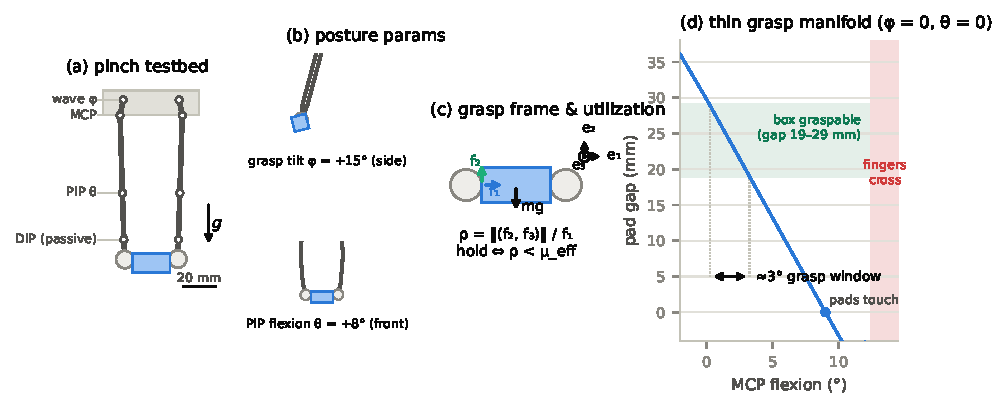
\includegraphics[width=0.76\textwidth]{figs/F1_setup.pdf}
  \caption{Simulation testbed. (a)~Two-finger hand with compliant
    hydroelastic fingertip domes, mounted fingers-down so gravity loads the
    pinch contacts in shear. (b)~Grasp frame built from the two contact
    centroids: squeeze $f_1$, weight-bearing shear $f_2$, lateral shear
    $f_3$; utilization $\rho = \lVert(f_2,f_3)\rVert / f_1$. (c)~The grasp
    manifold is thin: the pad gap sweeps its graspable band in
    ${\approx}3^\circ$ of MCP flexion, so postures are parameterized by
    grasp tilt $\phi$ and PIP flexion $\theta$ with MCP solved per
    condition.}
  \label{fig:setup}
\end{figure*}

\textbf{Hand and materials.} The testbed (Fig.~\ref{fig:setup}a) is a
two-finger hand (``Touch\_Finger'') with per-finger kinematic chain
wave~$\to$~MCP~$\to$~PIP~$\to$~DIP, mounted fingers-down so the pinch axis
is horizontal and gravity loads the contacts in shear. Wave, MCP, and PIP
are actuated (posture PD with gravity feedforward); DIP is passive, a
torsional spring toward the measured PIP angle (k = 0.35~N$\cdot$m/rad,
${\approx}5^\circ$ of give at 1--2~N). Fingertips are hemispherical domes
simulated as compliant hydroelastic solids (elastic modulus 50~kPa nominal,
Hunt--Crossley dissipation 1.5~s/m, $\mu_s/\mu_d = 1.2/0.9$); objects are
rigid hydroelastic ($\mu_s/\mu_d = 1.0/0.8$), giving a Coulomb pair
coefficient $\mu_d \approx 0.85$ (harmonic mean). The reference object is a
$25 \times 25 \times 12$~mm, 50~g block. Simulation uses Drake~1.54, SAP
solver, 2~ms steps for boundary trials and 1~ms for slip trials.

\textbf{Idealized tactile signal.} Per fingertip we read the hydroelastic
contact resultant force and patch centroid --- an idealized TacTip. From
the two centroids we build the grasp frame (Fig.~\ref{fig:setup}b): $e_1$
along the grasp axis (squeeze force $f_1$), $e_2$ vertical in the plane
normal to $e_1$ (the weight-bearing shear $f_2$),
$e_3 = e_1 \times e_2$ (lateral shear $f_3$). Utilization
$\rho = \lVert (f_2, f_3) \rVert / f_1$ is the fraction of a Coulomb budget
in use; classical analysis predicts failure at $\rho \approx \mupair$. The
slip detector is additionally evaluated on a 100~Hz sample-and-hold variant
of this signal, the camera rate of the physical sensor.

\textbf{Grasp acquisition and force control.} A state machine closes to a
posture, acquires contact, servos the squeeze component $f_1$ to a setpoint
(integral torque trim on MCP), releases the object's spawn support, and
holds. Gravity-compensation feedforward is required at tilted postures ---
without it, PD sag consumes the few-degree contact window.

\textbf{The grasp manifold is thin.} The pads oppose ${\sim}30$~mm apart at
zero flexion and the fingers physically cross a few degrees later
(Fig.~\ref{fig:setup}c): the pad gap sweeps its graspable band in
${\approx}3^\circ$ of MCP flexion. Postures are therefore parameterized by
\textbf{grasp tilt $\phi$} ($\pm 15^\circ$; a rigid rotation of the grasp
about the pinch axis that reorients gravity on the pads) and \textbf{PIP
flexion $\theta$} ($-5^\circ \ldots +10^\circ$), with MCP solved per
condition to hit a 24~mm pad gap.

\textbf{Boundary protocol.} For each condition $(\phi,\theta,\mathrm{mass})$
the minimal stable squeeze $\fstar$ is located by a mass-scaled ascending
force ladder followed by log-space bisection: 7 steps, 2 spawn seeds per
probe (stable only if \emph{all} seeds hold), ``stable'' = object drift
$< 2$~mm in the tip frame over a 3~s hold. The primary sweep covers 5 tilts
$\times$ 8 flexions $\times$ 3 masses (30/60/120~g) = 120 conditions,
${\approx}2{,}100$ trials. Three dedicated studies use stronger statistics:
shape/material tables use 5 seeds per probe, carried-grasp statistics 10
seeds, and a seed-noise audit (12 conditions $\times$ 5 independent
bisections) measures the seed-to-seed spread of $\fstar$ itself ---
2--7\,\% of the median at 30~g but 7--32\,\% at 60~g --- numbers that
become the weights and exclusions of \S\ref{sec:envelope}.

\section{The Stability Boundary Is Rolling-Governed}
\label{sec:rolling}

\begin{figure*}[t]
  \centering
  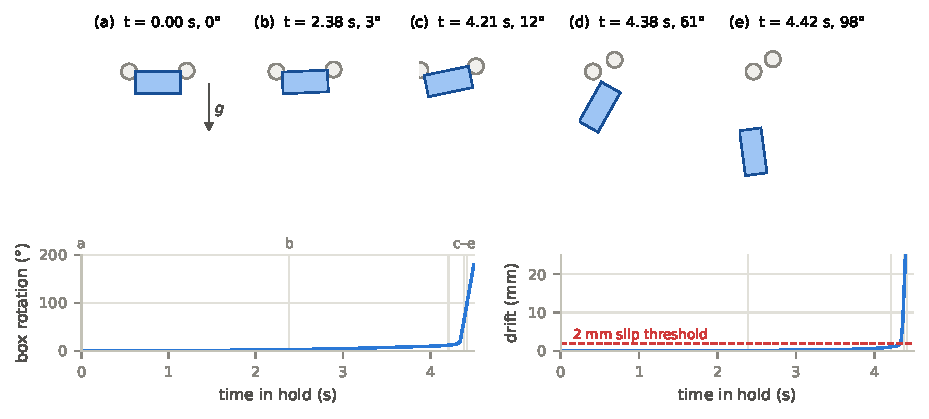
\includegraphics[width=0.74\textwidth]{figs/F2_rolling.pdf}
  \caption{Anatomy of the canonical failure: a 50~g block held at
    $1.3\times\fstar$. Drift stays under the 2~mm criterion for seconds
    while the block rotates at fractions of a degree per second; the
    rotation accelerates smoothly and the block rolls off the dome
    shoulders ${\sim}200$~ms later. At failure, utilization
    $\rho \approx 0.5$.}
  \label{fig:rolling}
\end{figure*}

\textbf{Failure looks like rolling, everywhere.} Fig.~\ref{fig:rolling}
shows the canonical failure: a 50~g block held at $1.3\times\fstar$ at the
reference posture. For five seconds drift stays under a millimeter while
the block rotates at fractions of a degree per second; the rotation
accelerates smoothly and the block is gone ${\sim}200$~ms later, tumbling
$176^\circ$. Translation --- the thing a Coulomb analysis watches --- stays
below the 2~mm threshold until the roll-off is already unrecoverable; at
failure, utilization $\rho \approx 0.5$, barely half the nominal friction
budget.

\textbf{The stability ratio never reaches Coulomb.} Define
$\mueff = (mg/2)/\fstar$, the value a friction-cone analysis would infer
from the measured boundary. If sliding governed, $\mueff$ would equal the
pair coefficient. Instead, across the friction sweep
(Table~\ref{tab:materials}, Fig.~\ref{fig:shapes}b), $\mueff/\mupair$
stays at 0.66--0.77 in the mid-to-high friction range: $\fstar$ follows the
Coulomb-like $1/\mu$ scaling --- friction sets the \emph{scale} --- but the
boundary binds 25--35\,\% early, at the roll-off.

\begin{table}[t]
  \caption{Material study: friction pair and fingertip stiffness (box
    object, reference posture, 5 seeds).}
  \label{tab:materials}
  \centering
  \setlength{\tabcolsep}{4pt}
  \resizebox{\columnwidth}{!}{%
  \begin{tabular}{lcccc}
    \toprule
    material variation & pair $\mu_d$ & $\fstar$ (N) & $\mueff$ &
      $\mueff/\mupair$ \\
    \midrule
    low friction (box $\mu_d$ 0.3) & 0.45 & \multicolumn{3}{c}{none ---
      window closed} \\
    base (box $\mu_d$ 0.8) & 0.85 & 0.435 & 0.564 & 0.66 \\
    high friction (box $\mu_d$ 1.2) & 1.03 & 0.311 & 0.789 & 0.77 \\
    soft tips, 25~kPa & 0.85 & 0.504 & 0.487 & 0.57 \\
    stiff tips, 100~kPa & 0.85 & 0.360 & 0.681 & 0.80 \\
    \bottomrule
  \end{tabular}}
\end{table}

\begin{table}[t]
  \caption{Shape study: geometry only (50~g, identical friction pair,
    25~mm grasp width, 5 seeds).}
  \label{tab:shapes}
  \centering
  \setlength{\tabcolsep}{4pt}
  \resizebox{\columnwidth}{!}{%
  \begin{tabular}{llcc}
    \toprule
    shape & contact type & $\fstar$ (N) & $\mueff$ \\
    \midrule
    disc, axis $\parallel$ grasp axis & flat round faces & 0.298 & 0.823 \\
    box $25{\times}25{\times}12$~mm & flat square faces & 0.435 & 0.564 \\
    prism $25{\times}50{\times}12$~mm & flat faces, $2\times$ lever arm &
      0.435 & 0.564 \\
    cylinder $d=25$~mm, axis vertical & curved rim & 0.464 & 0.529 \\
    disc on edge (key pinch) & rim, gravity on roll axis & 0.572 & 0.429 \\
    sphere $d=25$~mm & point contact & 0.596 & 0.411 \\
    \bottomrule
  \end{tabular}}
\end{table}

\begin{figure}[t]
  \centering
  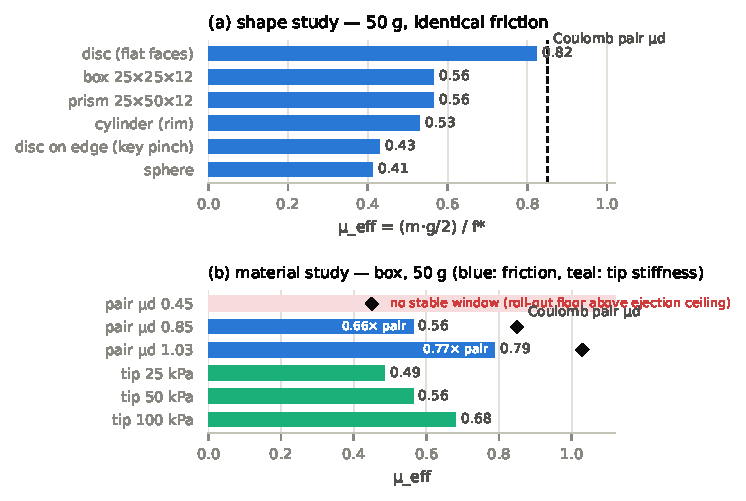
\includegraphics[width=\columnwidth]{figs/F3_shapes_materials.pdf}
  \caption{(a)~Shape study: $\mueff$ ordered exactly by the object's
    freedom to roll, spanning $2\times$ in $\fstar$ at identical Coulomb
    friction. (b)~Material study: $\mueff$ tracks but never reaches the
    pair coefficient (rolling discount $0.66$--$0.77$); softer tips are
    worse.}
  \label{fig:shapes}
\end{figure}

\textbf{Geometry alone spans $2\times$ at fixed friction.} The shape study
(Fig.~\ref{fig:shapes}a, Table~\ref{tab:shapes}) holds mass (50~g),
friction pair, and grasp width (25~mm) fixed and varies only geometry; the
ordering is exactly the object's freedom to roll: flat faces resist
rotation best, rims and points roll easily, and lateral prehension of a
disc is nearly worst (gravity torque acts directly about the free rolling
axis). Two details sharpen the mechanism. First, box and prism land on
\emph{exactly} the same bisection notch ($\fstar = 0.435$~N at 5-seed
resolution): doubling the lever arm about the grasp axis changes nothing,
so the flat-face boundary is set by the contact patch, not the object's
inertia. Second, the span disc~$\to$~sphere is $2.0\times$ in $\fstar$ ---
larger than the entire friction effect over the tested range --- at
\emph{identical} Coulomb friction. No friction-cone analysis, however
carefully calibrated, can reproduce this column.

\textbf{Softer fingertips are worse.} The naive expectation --- softer pad,
larger patch, more rolling resistance --- fails in the direction that
matters for sensor design: $\mueff$ falls from 0.68 (100~kPa) to 0.56
(50~kPa) to 0.49 (25~kPa). A compliant dome yields as the object rotates
and provides less restoring moment against rolling, so the skin softness
that maximizes tactile sensitivity directly taxes grasp stability --- a
quantified design trade-off for TacTip-class sensors.

\textbf{The friction picture can collapse entirely.} At pair
$\mu_d = 0.45$ the hold boundary (roll-off from below, 0.74~N) rises past
the ejection boundary (squeeze-out from above, ${\ge}1.5$~N): the stable
window is empty and \emph{no} squeeze force holds a 50~g box. Stability for
soft fingertips is a \textbf{window}, not a threshold --- its ceiling
(\S\ref{sec:envelope}) is as real as its floor.

\section{The Stability Envelope and a Minimal Grip-Force Rule}
\label{sec:envelope}

\begin{figure*}[t]
  \centering
  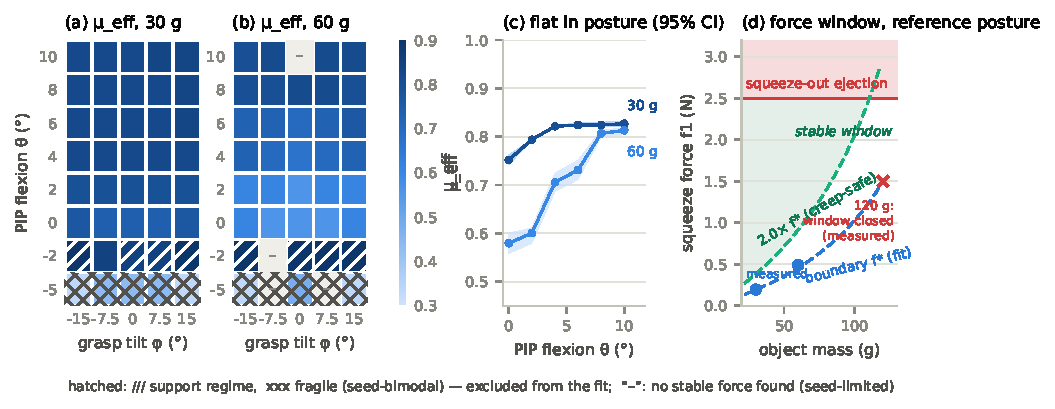
\includegraphics[width=0.76\textwidth]{figs/F4_envelope.pdf}
  \caption{The stability envelope. (a,b)~$\mueff$ maps at 30 and 60~g with
    automatically classified regimes: support band (///, $\fstar$
    mass-independent) and fragile band ($\times\times\times$, boundary
    existence seed-dependent) are excluded from the fit. (c)~The stable
    force window $[\fstar, {\approx}2.5~\mathrm{N}]$ narrows with mass and
    closes at 120~g.}
  \label{fig:envelope}
\end{figure*}

\textbf{The rule.} Inside the validity envelope established below, the
minimal stable squeeze force is
\begin{equation}
  f_1^{*}(m) = \frac{m g / 2}{\mueff}, \qquad
  \mueff \approx 0.71 - 4.2\,(m - 0.045)
  \label{eq:rule}
\end{equation}
with $m$ in kilograms. Mass, not posture, carries the rule. Bootstrap
confidence intervals over the fitted sweep (5{,}000 condition resamples)
retain only the intercept (0.707, 95\,\% CI $[0.674, 0.739]$) and the mass
slope ($-4.20$, CI $[-5.14, -3.20]$); every posture coefficient's CI
straddles zero. Inside the envelope, $\mueff$ is statistically flat in
posture; posture decides grasp stability at the \emph{regime boundaries}
(below), not inside the safe region.

\textbf{Descriptive posture refinement.} The full weighted-least-squares
fit over the \textbf{friction regime} ($n = 60$ conditions; regimes below),
in the physics form fixed a priori,
\begin{equation}
\begin{aligned}
  \mueff(\phi,\theta,m) ={}& 0.7069 - 0.0432\,\phi + 0.6019\,\theta \\
  & + 0.0959\,\phi^2 - 1.4668\,\theta^2 + 0.5369\,\phi\theta \\
  & - 4.1958\,(m - 0.045)
  \label{eq:quadratic}
\end{aligned}
\end{equation}
[$\phi,\theta$ in rad; $m$ in kg] uses per-mass weights from the audit's
measured seed noise and reaches $R^2 = 0.60$, RMSE $= 0.054$ over
$\mueff \in [0.56, 0.85]$ (unweighted OLS: $R^2 = 0.75$, over-weighting the
noisier 60~g rows). The explicit mass term --- $\mueff$ drops
${\approx}0.13$ per 30~g --- is essential: a posture-only fit collapses to
$R^2 \approx 0.36$. The strong PIP-flexion dependence suggested by the raw
map (Fig.~\ref{fig:envelope}a,b) is carried by rows the regime analysis
removes. Over the 16 held-out conditions \eqref{eq:rule} and
\eqref{eq:quadratic} differ by at most $+9\,\%/{-0.3}\,\%$ in predicted
$\fstar$ --- far inside the $0.6\times$--$1.25\times$ probe brackets --- so
the validation below applies to the one-line rule.

\textbf{Regimes (Fig.~\ref{fig:envelope}a,b).} Two bands are excluded from
the fit and reported separately, both detected automatically:
\begin{itemize}
  \item \emph{Support regime} ($\theta \approx -2^\circ$, hatched ///):
    the slightly-everted pads cradle the object and $\fstar$ becomes
    mass-independent (0.15--0.31~N for 30~$\to$~120~g, where Coulomb
    predicts proportionality). Classifier:
    $\fstar(2m)/\fstar(m) < 1.5$.
  \item \emph{Fragile regime} ($\theta = -5^\circ$, hatched
    $\times\times\times$): the boundary's \emph{existence} is
    seed-dependent --- 2/5 audit seeds cradle at
    $\fstar \approx 0.09$--$0.14$~N ($\mueff$ 1.6--2.2, above the Coulomb
    pair) and 3/5 find no stable force at all. These bimodal rows had
    carried the steep low-$\mueff$ end of earlier posture-only fits.
\end{itemize}

\textbf{The window and its ceiling (Fig.~\ref{fig:envelope}c).} Squeezing
beyond ${\approx}2.5$~N ejects the object from between the domes
(squeeze-out) regardless of posture. The stable window
$[\fstar, 2.5~\mathrm{N}]$ narrows with mass and at 120~g is empty at
nearly every posture: the pinch cannot robustly hold 120~g, and the fitted
mass term is validated only over 30--60~g.

\textbf{Held-out validation: 16/16.} Sixteen off-grid posture/mass points
inside the envelope (tilt up to $\pm 13^\circ$, flexion
$0.5^\circ$--$8.5^\circ$, masses 30--60~g) were each probed at $1.25\times$
and $0.6\times$ the predicted $\fstar$, two seeds per probe,
all-seeds-agree scoring: 32/32 probes correct. Three deliberate
out-of-envelope probes behaved as characterized: a fragile-band posture
held even at $0.6\times$ (cradling), 120~g dropped even at $1.25\times$
(window closed), and a 90~g probe passed --- the mass term extends usable
prediction at least somewhat beyond the fitted range.

\section{Slip Detection at the Sensor's Camera Rate}
\label{sec:slip}

\begin{figure*}[t]
  \centering
  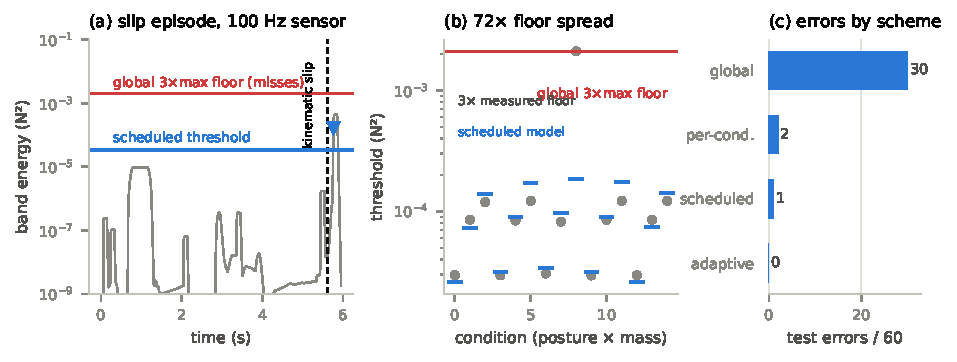
\includegraphics[width=0.74\textwidth]{figs/F6_slip.pdf}
  \caption{Slip detection at scale. (a)~A slip episode: the band-energy
    burst clears its own condition's pre-slip floor by ${\ge}3.6\times$.
    (b)~The floor varies $9\times$ (ideal rate) to $72\times$ (100~Hz
    camera rate) across the 15 posture~$\times$~mass conditions, so no
    global threshold works. (c)~Errors by calibration scheme: scheduling
    the threshold over $(\phi,\theta,m)$ recovers near-perfect detection at
    both rates.}
  \label{fig:slip}
\end{figure*}

A grip-force rule wants a safety net: detect incipient slip and bump the
setpoint. The detector is deliberately simple --- band energy (15~Hz
one-pole high-pass, 100~ms window) of the tangential force
$\lVert (f_2, f_3) \rVert$, thresholded --- and is evaluated against
kinematic ground truth (drift $> 2$~mm; sliding $> 5$~mm/s sustained
50~ms) at both the ideal simulation rate and the 100~Hz camera-rate
variant. A pilot at a single posture scores perfectly at both rates,
reproducing the common literature result; the deployable question appears
at scale: 90 episodes (45 induced slips, 45 clean holds) over 15 posture
$\times$ mass conditions spanning the envelope, split 30 train / 60 test:
\begin{itemize}
  \item \textbf{A single global threshold fails.} The pre-slip floor
    varies $9\times$ (ideal) to $72\times$ (camera rate) across
    conditions; the only safe global choice --- $3\times$ the maximum
    training floor --- misses every test slip (0~TP\,/\,30~FN), and even
    the oracle-best global threshold commits a false positive.
  \item \textbf{Detection itself is sound.} Within each condition, every
    slip burst clears that condition's own floor by ${\ge}3.6\times$
    (median $12\times$ ideal, $45\times$ camera rate); the broken piece is
    \emph{calibration transfer} across conditions
    (Fig.~\ref{fig:slip}a,b).
\end{itemize}

\textbf{Scheduled threshold.} Fit $\log_{10}$(pre-slip floor) over
$(\phi,\theta,m)$ on the training episodes --- the same scheduling recipe
as the grip-force rule --- and set the threshold to $3\times$ the predicted
floor. The floor model is modest ($R^2 = 0.48$ ideal, 0.68 camera rate) but
the ${\ge}3.6\times$ burst margin absorbs the prediction error
(Table~\ref{tab:slip}), matching the oracle-best global threshold with only
signals the controller already has (Fig.~\ref{fig:slip}c). A model-free
adaptive variant --- running-floor self-normalization with an absolute
noise guard and post-grasp arming --- reaches a perfect 30/0/0/30 at both
rates; its construction and ablations are documented in the released code.
Per-condition calibration (28/0/2/30) remains a diagnostic upper bound but
assumes training data at every operating condition --- precisely the
assumption scheduling removes. Camera-rate operation costs essentially
nothing: the floor \emph{spread} worsens but burst separability
\emph{improves}, because sample-and-hold decimation suppresses the
broadband floor more than the slip burst.

\begin{table}[t]
  \caption{Scheduled-threshold slip detection on the 60-episode test set
    (30 slip, 30 clean-hold). UB = 95\,\% upper bound.}
  \label{tab:slip}
  \centering
  \setlength{\tabcolsep}{3pt}
  \resizebox{\columnwidth}{!}{%
  \begin{tabular}{lccccccc}
    \toprule
    rate & TP & FP & FN & TN & latency & miss (UB) & FP (UB) \\
    \midrule
    ideal (1~kHz) & 30 & 1 & 0 & 29 & 0.168~s & 0\,\% (10\,\%) &
      3.3\,\% (${\approx}13$\,\%) \\
    camera (100~Hz) & 30 & 1 & 0 & 29 & 0.170~s & 0\,\% (10\,\%) &
      3.3\,\% (${\approx}13$\,\%) \\
    \bottomrule
  \end{tabular}}
\end{table}

\section{Carried Grasps and the Time Dimension}
\label{sec:carried}

\begin{figure}[t]
  \centering
  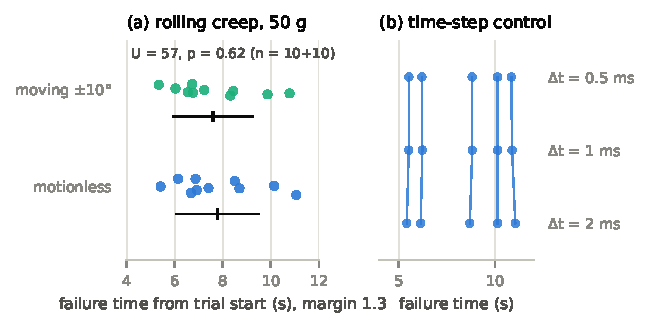
\includegraphics[width=0.92\columnwidth]{figs/F5_creep.pdf}
  \caption{(a)~Creep failure-time distributions at margin 1.3: motionless
    vs.\ carried holds, 10 seeds each; we detect no difference
    (Mann--Whitney $U = 57$, $p = 0.62$). (b)~Time-step control: 1~ms and
    0.5~ms steps reproduce each seed's failure time to within 0.04~s.}
  \label{fig:creep}
\end{figure}

\textbf{The boundary is hold-duration-dependent.} Carrying the 50~g box
through a grasp tilt sinusoid ($\pm 10^\circ$, 0.15~Hz, 2 cycles) at
$1.3\times\fstar$ fails --- and so does a motionless hold at the same
force. With 10 seeds per condition, margin 1.3 fails 20/20 runs, and the
failure time is a distribution, not a constant: 5.4--11.1~s motionless
($7.8 \pm 1.7$~s) versus 5.3--10.8~s carried ($7.6 \pm 1.6$~s). We detect
no difference between the distributions (Fig.~\ref{fig:creep}a;
$n = 10$ per group resolves only large differences), and the failure times
are insensitive to carry amplitude --- the motion is not what kills the
grasp. The mechanism is the rolling creep of Fig.~\ref{fig:rolling}: a
grasp that passes any fixed-duration test just above $\fstar$ still escapes
on the 5--11~s scale, with almost no tangential vibration until roll-off is
imminent --- no detector can rescue a grasp commanded at margin 1.3.

\textbf{The creep is physics, not solver drift.} Rerunning five motionless
margin-1.3 holds at 1~ms and 0.5~ms time steps reproduces each seed's
failure time to within 0.04~s (Fig.~\ref{fig:creep}b): the failure time is
converged with respect to the time step in the hydroelastic model.

\textbf{Design rule.} Command
$f_1 = 2.0 \times (mg/2)/\mueff$
for sustained holds and slow manipulation. At this margin, 30/30 seeded
carry runs (10 seeds $\times$ three controllers: fixed force,
map-scheduled, scheduled + vibration reflex) complete the full posture
sweep with ${\le}0.85$~mm drift; the 1.3 margin is trustworthy only for
holds ${\lesssim}4$~s. Along the
tested trajectory the fitted $\mueff$ is nearly flat in tilt, so scheduling
${\approx}$~fixed force by design there; the scheduled controller earns its
keep near regime boundaries. (Phase-B forces used a pre-revision fit; under
the final equation the margins are ${\approx}2.1$ and ${\approx}1.4$ ---
conclusions unchanged.)

\section{Limitations and Conclusion}
\label{sec:limitations}

\textbf{Limitations.} (i)~The tactile signal is an idealized TacTip --- the
hydroelastic contact resultant and centroid; real marker-flow force
estimates add noise, hysteresis, and calibration error, and the 100~Hz
variant bounds only the rate effect. Hardware validation, following the
sim-to-real path demonstrated for TacTip-class sensors
\cite{lin2022tactilegym2}, is the natural next step. (ii)~Boundary trials
at 2~ms Nyquist-limit vibration content to 250~Hz; slip trials use 1~ms.
(iii)~The 2~mm~/~3~s stability criterion itself defines $\fstar$, and
\S\ref{sec:carried} shows the boundary moves with hold duration; the
$\times 2.0$ rule is the duration-robust statement. (iv)~Sweep boundaries
use 2 seeds per probe and are seed-limited at 60~g (spread to 32\,\%).
(v)~A perfect 30~+~30 slip score still only bounds each error rate below
${\sim}10\,\%$ (rule of three); the floor model and adaptive constants are
tuned to this hand/object envelope. (vi)~One grasp width (25~mm) and one
base material pair; masses validated 30--60~g; the material study gives
scaling to other pairs only at the reference posture.

\textbf{Conclusion.} For soft tactile fingertips, the minimal-grip-force
question is not a friction question. The stability boundary is set by
rolling: it binds 25--35\,\% below the Coulomb limit at every friction
tested, moves $2\times$ with shape at fixed friction, worsens as fingertips
soften, and --- near the boundary --- depends on how long you intend to
hold. All of this is invisible to a friction-cone analysis and all of it is
capturable: a one-line mass-dependent rule with a measured envelope
predicts held-out boundaries 16/16, a posture-scheduled threshold makes a
simple vibration detector deployable at the sensor's real frame rate, and a
$\times 2.0$ margin converts the rule into a controller that did not drop
an object in 30 seeded carries --- every number reproducible from the
released code and data.

\balance
\bibliographystyle{IEEEtran}
\bibliography{refs}

\end{document}
